\subsection{Current measurement}
\label{sec:method_current}
This section shall describe the thought process and functionality of the current measurement part of the project.

\subsubsection{Idea}
As mentioned, we decided very early on that we wanted the current measurement as an extra feature for our product. The question then was, what methods were available to do this kind of measurement?
The two main categories of current measurement techniques we looked into were:
\begin{itemize}
    \item Voltage created over a known resistor
    \item Magnetic field created by current flowing through a coil
\end{itemize}

Before deciding, we first went on the easiest test, at least access-wise, which was voltage over a known resistor. This was done by designing a differential amplifier with an operational amplifier.
\begin{figure}[h]
    \centering
    \frame{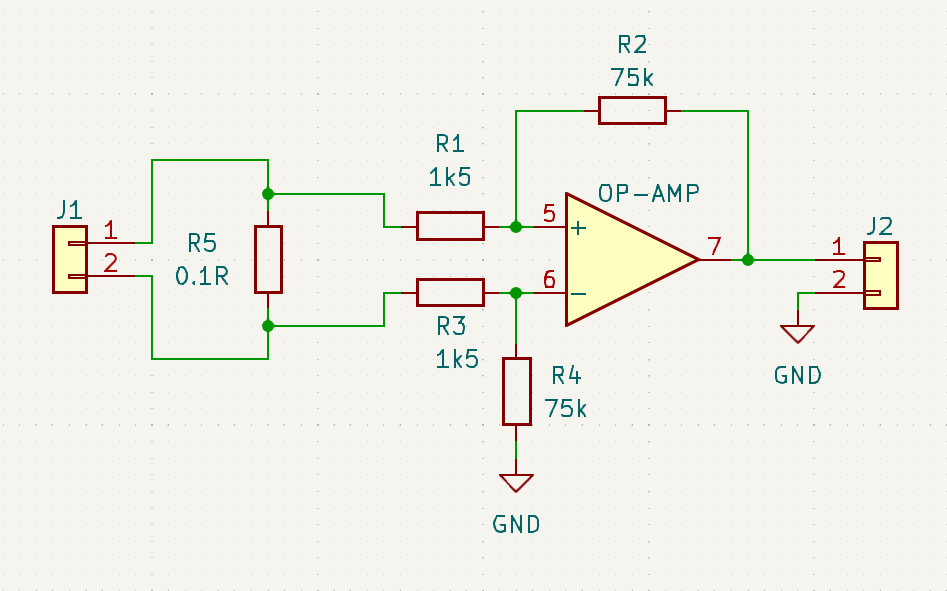
\includegraphics[width=\textwidth]{images/sch.diff.amp.png}}
    \caption{Differential amplifier used for testing}
    \label{fig:diff}
\end{figure}

As seen in Figure \ref{fig:diff}, the differential amplifier is built up by four resistors, the op-amp, and the shunt-resistor. This amplifier intends to magnify the voltage across the shunt-resistor, so the ADC in the Arduino can measure and then calculate the current flowing through the shunt, with the gain in mind.  The gain, in this case, was determined to be 50gg since our goal was a max current of 1A, and with a shunt resistance of 100m$\Omega$, this would result in an output of the amplifier to be 5V, which is the max input voltage. The gain was calculated with this equation, simplified:
\[V_{out}=(R_1/R_2)*(V_2-V_1)\]
Where the ratio between $R_1$ and $R_2$ is the overall gain and $V_2-V_1$ is the voltage difference that is multiplied.
\\
With this setup, we quickly discovered a limitation with this method, since there are special requirements for what is called a low-side measurement and a high-side measurement (Figure \ref{fig:hsls}). With the low-side measurement, this technique proved great, since this op-amp was an \textit{LM358APE4}, which has a very low common-mode voltage range that is ideal in this situation\footnote{See TI Application brief, References \ref{sec:references}}.

\begin{figure}[h]
    \centering
    \frame{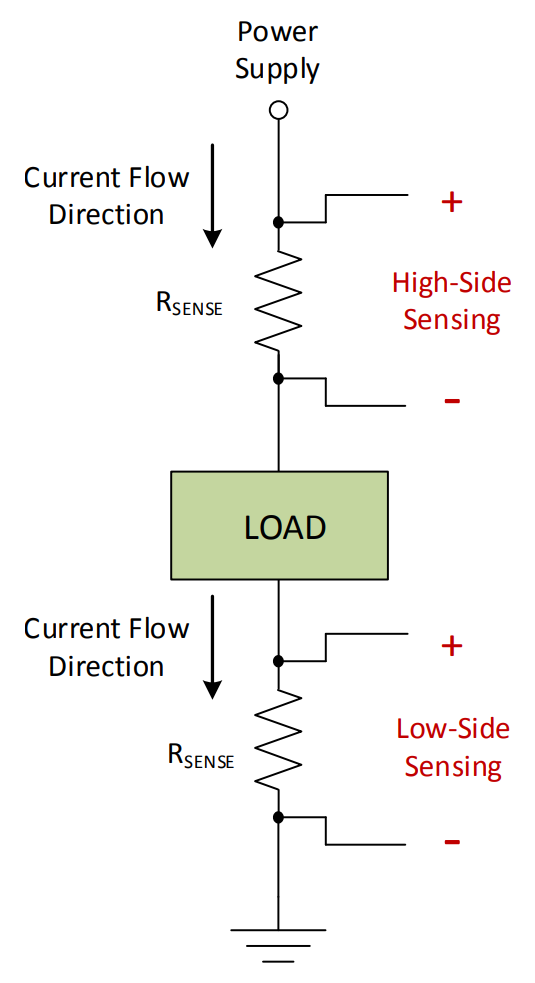
\includegraphics[scale=0.25]{images/hs_ls.png}}
    \caption{Specifying low-side versus high-side}
    \label{fig:hsls}
\end{figure}

But the opposite is the case with the high-side sensing, since in this instance the $V_{CM}$ is source dependent and thus can require a higher $V_{CM}$. This was where we decided on the other alternative to voltage over a known resistor. Because, with a multi-meter, you sometimes have to measure high-side and sometimes low-side, but the result can not be great if both considerations are implemented in the same design, since this would be paradoxical for an op-amp to have both properties.
\newpage
The current sensing method we then went with was the before-mentioned current through a coil. When this is the case, a magnetic field is created, and the magnitude of this field determines the current flowing through it. The limitations then are:
\begin{itemize}
    \item The thickness of the coil wire
    \item Saturation of the magnetic field
    \item Amount of winding
    \item Core material
\end{itemize}
And a way to measure the magnetic field.
With enough time to fine-tune these elements, this could be possible to implement ourselves, but we decided on buying an IC that would cover the whole spectrum with known elements.

\subsubsection{Implementation}
With the decision to go with an integrated circuit, the next step was to choose the sensor. With the limitation being the integrated ADC of the \textit{ATMEGA328}, we were looking for an analogue module, meaning the output voltage had to have a proportionality with the current. This voltage should have a high correlation with the current since we only have a 10-bit ADC.
\\ \\
We found a match on RS Components, mainly the \textit{ACS723LLCTR-05AB-T}. With the sensitivity being 400mV per 1A, this was the largest available. At the zero current, the output equates to $\frac{V_{CC}}{2}$, since this sensor is bidirectional in this case, 2.5V at 5V$_{CC}$. The \textit{ACS723} has a maximum current rating of 5A, at this current the max output voltage corresponds to 
\[V_{offset}+(V_{sens}*A)=V_{out}\Rightarrow2.5V+(0.400V*5)=4.5V\]
 The same is the case at -5A, hence 
\[2.5V+(0.400V*(-5))=0.5V\]
% \newpage
The magnetic field sensor used in this IC is a chopper-stabilized BiCMOS Hall IC. As illustrated by Figure \ref{fig:currentSens}\footnote{Illustration by Monolithpower, see References \ref{sec:references}} the conductor will generate a magnetic field, that is then picked up by the Hall transducer, and then amplified. 
\begin{figure}[h]
    \centering
    \frame{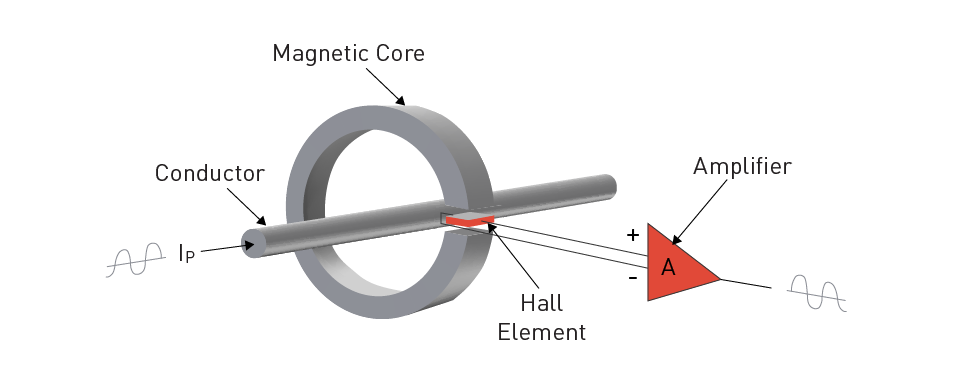
\includegraphics[width=\textwidth]{images/Current_Sensors_Article_Fig5-_960_x_385.png}}
    \caption{Current sens illustration}
    \label{fig:currentSens}
\end{figure}
\\
Another great feature of having this kind of sensor is the galvanic isolation between the two circuits, meaning the circuit measured cannot destroy or advisedly interfere with our system and vice versa. The only real interference when measuring a circuit would be the impedance introduced with IC, typically 0.65m$\Omega$ - basically nothing.

The \textit{ACS723} also has a tuned filter implemented that can be programmed by external components via its bandwidth select pin (6). If it is pulled down to GND, it selects the 80kHz range, while pulled up the filter is selected to be 20kHz. Since we can not utilize this extra bandwidth, and after some testing, we chose the 20kHz range by pulling it up to $V_{CC}$.
% \newpage
\begin{figure}[h]
    \centering
    \frame{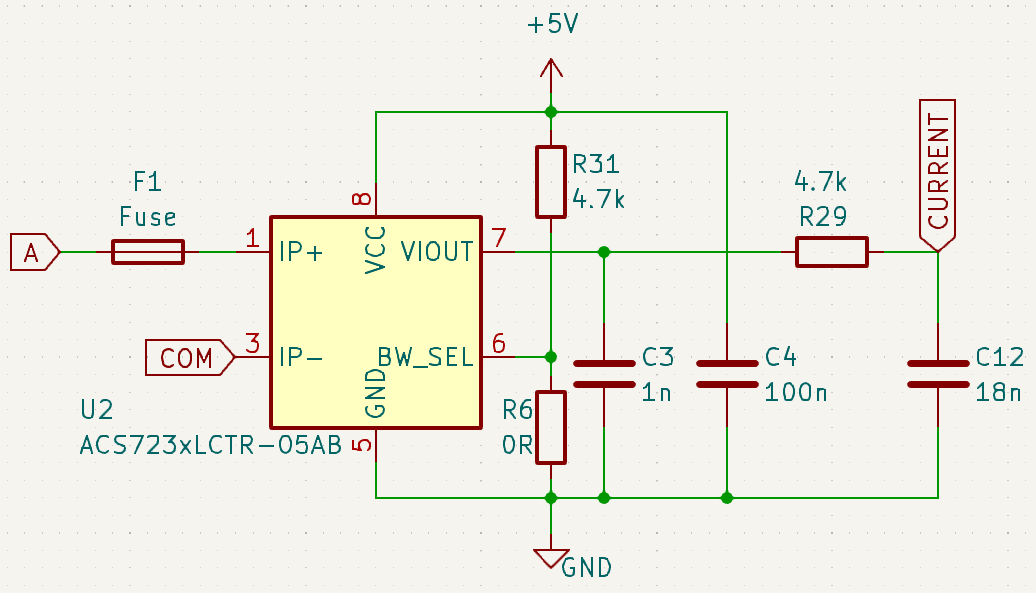
\includegraphics[width=\textwidth]{images/Current_sch.png}}
    \caption{Current sense schematic}
    \label{fig:CurrSch}
\end{figure}

For the circuit of the current sensor, see Figure \ref{fig:CurrSch}, we implemented a fuse of 5A and a low-pass filter. The filter is based on the sampling frequency of 20kHz mentioned before, to filter out unwanted noise. The dampening equates to -20dB since we used 2kHz as our cut-off frequency. With a predetermined resistor of 4.7k$\Omega$, we only need to determine the capacitor, in this case, C12
\[C_{12}=\frac{1}{2\pi*f_0*R}\Rightarrow\frac{1}{2\pi*2*10^3Hz*4.7*10^3\Omega}=16.9*10^{-9}F\Rightarrow18nF\]
With this 1$^{st}$-degree filter, the dampening equates to -20dB/decade, hence each doubling of frequency is a dampening of a factor of 10. Any higher frequencies picked up will be grounded by the capacitor.
\\\\
The fuse, F1, will be of a 5x20mm flick-type or F-type, meaning it will interrupt- or burn over quickly when it reaches 5A and not linger - thus fast-acting, to minimize the damage it might cause the IC. It is mounted on a PCB fuse block, thus making it easy to change.
% \newpage
\subsubsection{Code}
The code is set so the voltage we read from the \textit{ACS723} right when we switch to the function, via the buttons, is set as the voltage reference. This equates to about 2.5V but can vary quite a lot from time to time, $\pm$50mV, so it was necessary to measure the voltage at zero current draw, to the reference voltage. The voltage is sampled 100 times in the for-loop to remove unnecessary noise. With the known sensitivity of 400mV/A, and 10-bit ADC sampling, the current can be calculated, where \textit{value} is the filtered measured voltage from the loop:

\begin{align}
  & currFactor      &= &\hspace{2mm} \frac{1000}{400}                 &\text{(Sensitivity)} \notag \\
  & shuntVoltage    &= &\hspace{2mm} \frac{5}{1023}*1000*value       &\text{(ADC 10-bit value to voltage)} \notag \\
  & current         &= &\hspace{2mm} (shuntVoltage-V_{ref})*currFactor   &\text{(Actual current)} \notag \\
  \notag
\end{align}
